\documentclass[a4paper,12pt]{report}
\usepackage[english]{babel}
\usepackage{amsmath}
\usepackage{graphicx}
\usepackage{lscape}
\usepackage{rotating}
\usepackage{longtable}
%\usepackage[authoryear]{natbib}
\usepackage[numbers]{natbib}
\usepackage{hyperref}
\usepackage{subfig}
\usepackage{url}
\usepackage[a4paper]{geometry}

\begin{document}
% Row images for full page comparison
\newcommand{\imagerow}[2]{
\begin{minipage}{\textwidth}
    \centering
    \raisebox{-0.5\height}{\includegraphics[width=0.10\textwidth]{figures/logos/#2.pdf}}
    \hspace*{0.01\textwidth}
    % trim is left bottom right top
    \raisebox{-0.5\height}{\includegraphics[height=0.25\textwidth,trim=30 20 35 30,clip]{figures/notebooks/#1/even-#2.pdf}}
    \hspace*{0.01\textwidth}
    \raisebox{-0.5\height}{\includegraphics[height=0.25\textwidth,trim=30 20 35 30,clip]{figures/notebooks/#1/uneven-#2.pdf}}
\end{minipage}
}

% Full page comparison
% First argument is directory location, also used as reference name for label.
% Second argument is the caption
\newcommand{\onepagecmp}[2]{
\newgeometry{top=0.1cm,left=0.1cm,right=0.1cm,bottom=0.1cm}
\begin{figure}[p]
\centering
\thispagestyle{empty}
%\vspace{-2cm}
\begin{minipage}{\textwidth}
    \hspace*{0.16\textwidth}
    \centering
    \raisebox{-0.5\height}{
\includegraphics[width=0.10\textwidth]{figures/logos/even.pdf}}
    \hspace*{0.25\textwidth}
    \centering
    \raisebox{-0.5\height}{
\includegraphics[width=0.10\textwidth]{figures/logos/uneven.pdf}}
\end{minipage}
\imagerow{#1}{contig}
\imagerow{#1}{contig-merge}
\imagerow{#1}{scaf}
\imagerow{#1}{contig-scaf}
\imagerow{#1}{contig-merge-scaf}
\parbox{6in}{\caption{#2\label{fig:#1}}}
\end{figure}
\restoregeometry
}


\title{MSc Thesis - Benchmark of {\em de novo} Short Read Assembly Strategies for Metagenomics}
\author{Ino de Bruijn\\ {\bf Supervisor:} Assistant Prof. Anders Andersson}

\maketitle

\tableofcontents

\chapter{Introduction}
% random comment
Metagenomics, the sequencing of environmental DNA, has demonstrated to be a
promising approach for the discovery and investigation of microbes that cannot
be cultured in the laboratory \cite{Eisen17355177} as well as for the study of
both free-living microbial communities \cite{Andersson18497291} and microbial
communities inside other organisms \cite{Qin20203603,Hess21273488}.\\


In a typical shotgun metagenomics experiment the DNA of a community is isolated
and high throughput sequencing is performed on a random sample of the isolated
DNA \cite{Morgan20419134}. The reads can either be analyzed as such, by e.g.
blast searches against reference databases to obtain a functional profile of
the microbial community \cite{Tringe15845853}, or they can be assembled to form
longer stretches of DNA stemming from the same or closely related organisms
that can subsequently be analyzed with regards to phylogenetic affiliation and
functional properties. The output of the assembly process often includes
scaffolds, contigs and unassembled reads \cite{Mavromatis17468765}. One of the
problems with assembling is that chimeric contigs or scaffolds may be formed.
Closely related sequences are more likely to form chimeras and since closely
related strains often occur in the same environment this is a challenge. Also,
it is difficult to determine whether the formation of a chimera is natural due
to homologous recombination or an error in the assembly process
\cite{Tyson14961025}. Another problem with assembly is variations in gene
content among closely related strains, since a gene inserted in a subpopulaton
will cause conflicting assembly results \cite{Hallam17114289}. After assembling
the reads, a process called binning is performed, where the resulting scaffolds
and contigs are assigned to phylogenetically related groups. Finally, gene
calling and functional annotations are performed on the scaffolds.\\

% rewrite upper part (maybe take some parts from theoretical background)

In our studies several strategies for {\em de novo} assembly of metagenomic
data have been evaluated. In an {\em in silico} performed comparison between
Illumina, Sanger and 454 on cost of sequencing and resulting coverage of
microbial communities, Illumina short read libraries were shown to be the best
for communities of medium complexity \cite{Mende22384016}. Therefore we have
chosen to assess the assembly strategies for Illumina paired short reads
sepecifically.  In previous studies mostly {\em in silico} metagenomic data
sets have been used \cite{Pignatelli21625384,Mavromatis17468765}. In contrast
the community of our study is an {\em in vitro} simulated metagenome consisting
of 59 species with completed or nearly completed genomes so the quality of our
assesment is not dependent on the realisticness of read simulators. An even and
uneven distribution of the 59 species were created in vitro. The community has
been sequenced with different type of library preparations to be able to test
the difference in library preparation as well.  The following assembly programs
have been tested: Velvet \cite{Zerbino18349386}, Meta-Velvet \cite{MetaVelvet},
Newbler \cite{Quinn18755037}, Minimus2 \cite{Sommer17324286}, Ray Meta
\cite{Boisvert23259615} and Bambus2 \cite{Koren21926123}. The quality of the
assemblies have been evaluated by mapping the constructed contigs or scaffolds
to the collection of reference genomes, hereafter referred to as the reference
metagenome. In addition two pipelines have been constructed, one to perform the
assemblies and another to perform the validation given there is a reference
metagenome available.

%\chapter{Theoretical Background}
%% maybe mention some general paper overview of different assembly methods
%% PRactical ZHang de novo genome assembly).
%%Studying microbes in their natural environment is difficult for a number of reasons. One obvious
%%reason is that their size makes field studies impractical. A way around this
%%issue is culturing microbes in the laboratory. Unfortunately the vast majority of
%%microbes have not successfully been cultured in the lab \cite{Eisen17355177}.
%%By isolating the DNA of a community and sequencing that, analysis of a
%%community $in vivo$ can be performed. The most popular methods for sequencing
%%DNA from a sample of microbes are Illumina paired end and 454 sequencing (TODO:
%%citations). The sequencing process results in short reads of around 100 bp for
%%Illumina HiSeq and around 400 bp up to 1 kbp for 454 GS FLX Titanium (TODO:
%%citations). After sequencing the reads can be mapped against a reference
%%database of the same or closely related organisms to get a functional profile
%%of the community. Assembling the reads into longer contiguous segments of DNA
%%(contigs) before functional analysis has however been shown to improve the
%%accuracy (TODO: citations). 
%
%
%There are mainly three different categories of assembly approaches:
%Greedy-extension, de Bruijn graph and Overlap-Layout-Consensus (OLC)
%\cite{Zhangdadad}. Greedy-extension is a string-based method and the latter two
%use graphs.

\chapter{Related Work}
% Start with success of single genome evaluation, continue to metagenomic

In a study by \citet{Mavromatis17468765} three genome assemblers were
evaluated: Phrap \cite{delaBastide18428783}, Arachne \cite{Batzoglou11779843}
and Jazz \cite{Aparicio12142439}. For the evaluation three artificial
communities were constructed of low, medium and high complexity by selecting
Sanger reads from 113 isolate genomes. The low complexity community had one
dominating population with several low-abundance ones, the medium more than one
dominating population and the complex community had no dominating population at
all. Resulting contigs were evaluated on chimericity and length distribution.
Compared to using the original reads for gene annotation, assembly was
demonstrated to give up to 20\% increase in accurate gene prediction
and a slightly better increase for inaccurate and missed genes. Sanger reads of
700 bp were used. This approach of using artificial communities has
subsequently been used in adapted versions by several other assembly evaluation
papers \cite{Pignatelli21625384,Mende22384016}. In the benchmark by
\citet{Pignatelli21625384} the reads of the artificial communities were changed
from Sanger to 454 and Illumina. For the Illumina reads, SSAKE
\cite{Warren17158514} and Velvet were used to perform the assembly. No
difference in chimericity between using the simulated 454 reads or the Illumina
reads was spotted. The main cause of chimericity was sequence similarity of the
organisms, no relation with genome coverage was found. At the functional level
metagenomic assembly turned out to be counterproductive compared to using the
original reads for annotation. \citet{Mende22384016} used a metagenome of 10,
100 and 400 species with simulated reads of Illumina, 454 and Sanger where the
number of reads for each technology was based on sequencing cost. The
sequencing cost was kept constant. All of the technologies provided similar
coverage for 10 species. Illumina was superior for 100 species due to the
higher coverage one can get for a similar price.  Sanger performed best for 400
species because of longer read length. Sanger reads were assembled with
Arachne; 454 reads with Celera \cite{Myers10731133} and Illumina reads with
SOAPdenovo \cite{Li20019144}. Similar to the study of
\citet{Pignatelli21625384} a year earlier, the authors concluded that assembly
contigs improves functional annotation of the metagenome. Furthermore using
Illumina paired end data to determine contig links and construct scaffolds,
although introducing more chimerism, resulted in an even better functional
annotation.  Beyond using simulated reads or real reads of {\em in silico}
communities there has not been a comparison of assembly algorithms using an
{\em in vitro} community yet.  In vitro communities have been used previously
with success to assess DNA extraction techniques for sequencing a low
%TODO find number of genomes
complexity community of nine bacterial genera \cite{Willner22514642}, an oral
community \cite{Diaz22520388}, the human gut \cite{Wu20673359} and the human
microbiome \cite{HMPC22699610}.  The advantage of using an {\em in vitro}
community for assembly evaluation is that one does not have to rely on the
correctness of sequencing simulators, the assessment can thus be as good as the
similarity of the {\em in vitro } community to a real community.

%Say something about GAGE and Assemblathon

\chapter{Methods and Materials} To determine the quality of metagenomic assembly a mock
community of species with known genomes was constructed {\em in vitro} and
sequenced with Illumina. The resulting reads have been assembled using a
combination of Velvet, Meta-Velvet, Ray, Minimus2, Newbler and Bambus2 resulting in
nineteen different assembly strategies (see Figure \ref{fig:asmstrat} and Table
\ref{tab:asmstrat}). The strategies stem from current literature and our own
ideas.

\section{Mock community} The mock community consists of 49 bacterial and 10
archaeal species with finished or nearly completed genomes (Table
\ref{tab:mock}). The species have been chosen such that there are a number of
closely related organisms and more distant ones. The number of species is about
equal to the number of species one would find in the human gut. The abundances
of DNA from each species have been fixed in two types of configurations before
sequencing. In the first configuration, the even configuration, all species
have approximately equal genome copy numbers. In the second configuration, the
uneven configuration, the phyla are mixed in proportions similar to log-normal
distributions of phyla in soil \cite{Doroghazi18682841}. The samples have been
prepared with the Nextera 50ng sample preparation kit. The entire reference
metagenome's size is about 195Mb. Mock community preparations and sequencing
were performed by our collaborators, Christopher Quince at University of
Glasgow and Linda D'Amore and Neil Hall at Liverpool's Centre for Genomics
Research.

% The V3 (192 bp) and V4 (291 bp) of the 16S genes have been amplified and the samples have been sequenced with Illumina.

\section{Quality trimming} Before assembling the reads one often starts with
pre-processing them by quality trimming and/or removing PCR duplicates.
\citet{Mende22384016} demonstrated that quality trimming could drastically
improve the assembly. Before each assembly the same quality trimming procedure
has been performed. For quality trimming the program sickle was used (see Table
\ref{tab:programversions}). Reads were trimmed from the 3' end if the average
quality score was below 20 in a window of 10 bases. If the resulting read is
shorter than 20 it is discarded. Only pairs are used in the subsequent
assembly, not the single reads.


\section{Assembly} In the assembly procedure reads are combined into
contiguous sequences called contigs. Contigs can afterwards be joined using
paired read information into longer scaffolds. In the scaffolding process
contigs might be extended and repeats might be solved so scaffolding is not
restricted to just the ordering of contigs.\\


There are a plethora of different assemblers available and by pre-processing
reads and combining different assemblers an even larger amount of assembly
strategies is possible. Velvet is one of the most used assembly programs and
was therefore included in this assessment. Velvet's metagenomic counterpart,
Meta-Velvet, is performed after executing Velvet so it is possible to determine
how the metagenomic specific parameters improve the assembly. Another popular
assembler that has recently received an update for metagenomics is Ray (TODO:
cite). Ray is based on MPI and is runnable over multiple nodes distributing
both memory and processor load, which makes it an ideal candidate for large
metagenomic projects.\\


\subsection{Contiging}
Velvet, Ray and Meta-Velvet all use a de Bruijn graph to determine overlaps
between reads. This involves cutting up the reads in sizes of a specified kmer
size and let edges represent overlaps between kmers i.e. ($k+1$)mers. This way
the graph, or the computational requirements, grow with the number of unique
kmers in the library instead of the number of reads. For a more elaborate
description of de Bruijn Graphs for sequence assembly see
\cite{Miller20211242}. The resulting contigs are constructed by following paths
in the graph. The paths that can be unambiguously followed are called unitigs.
Ambiguous paths can be solved by using coverage information or paired-end
information. Contigs thus consist of one or multiple unitigs. Choosing the
right kmer size is important. A shorter $k$ gives more connectivity within the
graph and hence requires lower sequencing coverage of the genomes, but at the same
time the risk increases that a kmer occurs multiple times within a genome,
or in multiple genomes (hence ambiguous paths will exist). A larger $k$ can overcome this problem if it is larger
than the multiply occurring region. But a larger $k$ also requires higher
sequence coverage.\\


\subsubsection{How the assemblers differ}
Velvet, Ray and Meta-Velvet differ in the way the graph is traversed. Velvet,
meant for single genomes, looks for one coverage peak in the coverage
distribution and tries to follow that, where the main idea is that the genome
is approximately uniformly covered. Nodes in the graph below a certain coverage
threshold are considered errors and ones with high coverage repeats.
Meta-Velvet looks for multiple peaks in the coverage distribution. The contigs
of each genome
should have a distinct coverage peak due to the genome copy number of the
corresponding genome being different from the other genomes in the metagenome. Meta-Velvet
makes use of that property. Ray looks for 'seeds' in the graph and extends
those seeds iteratively weighting choises by the number of reads supporting a
certain path. The seeds are unitigs in the graph with a specific coverage. The
metagenomic update to Ray changes the seed selection by looking at the coverage
peak in the graph locally instead of globally. 


\subsection{Merging}
A way to get the advantage from both short and long kmers is by merging contigs
generated in multiple assemblies with different kmer lengths. This is possible
with Newbler, as done by \citet{Luo22347999}, or with Minimus2, as done by for
instance the Rnnotator pipeline \cite{Martin21106091}. Both Newbler and
Minimus2 use an Overlap-Layout-Consensus method to merge contigs
\cite{Sommer17324286,Miller20211242}.


\subsection{Scaffolding}
For the scaffolding procedure Bambus2 was chosen since it was one of the better
scaffolders for single genomes in the GAGE assessment paper
\cite{Salzberg22147368} and is suitable for metagenomes as well
\cite{Koren21926123}. For a flow diagram of previously mentioned approaches see
Figure \ref{fig:asmstrat}. A total of twelve assembly strategies from the flow
diagram have been tested. See Table \ref{tab:asmstrat} for an overview of the
assembly strategies, Table \ref{tab:programversions} for versions of each
program and Table \ref{tab:asmstratparameters} for the parameters of each
strategy.


\begin{table}[h!]
\centering
\begin{tabular}{|l|c|c|c|}
\hline
Assembly strategy name & Contiging & Merging & Scaffolding\\
\hline
velvetnoscaf & Velvet & - & -\\
velvetscaf & Velvet & - & Velvet\\
minimus2velvetnoscaf & Velvet & Minimus2 & -\\
newblervelvetnoscaf & Velvet & Newbler & -\\
bambus2velvetnoscaf & Velvet & - & Bambus2\\
bambus2minimus2velvetnoscaf & Velvet & Minimus2 & Bambus2\\
bambus2newblervelvetnoscaf & Velvet & Newbler & Bambus2\\
metavelvetnoscaf & Meta-Velvet & - & -\\
metavelvetscaf & Meta-Velvet & - & Meta-Velvet\\
minimus2metavelvetnoscaf & Meta-Velvet & Minimus2 & -\\
newblermetavelvetnoscaf & Meta-Velvet & Newbler & -\\
bambus2metavelvetnoscaf & Meta-Velvet & - & Bambus2\\
bambus2minimus2metavelvetnoscaf & Meta-Velvet & Minimus2 & Bambus2\\
bambus2newblermetavelvetnoscaf & Meta-Velvet & Newbler & Bambus2\\
raynoscaf & Ray & - & -\\
rayscaf & Ray & - & Ray\\
minimus2raynoscaf & Ray & Minimus2 & -\\
newblerraynoscaf & Ray & Newbler & -\\
\hline
\end{tabular}
\caption{Assembly strategies}
\label{tab:asmstrat}
\end{table}

\clearpage
\thispagestyle{empty}
\begin{figure}[ht!]
  \centering
    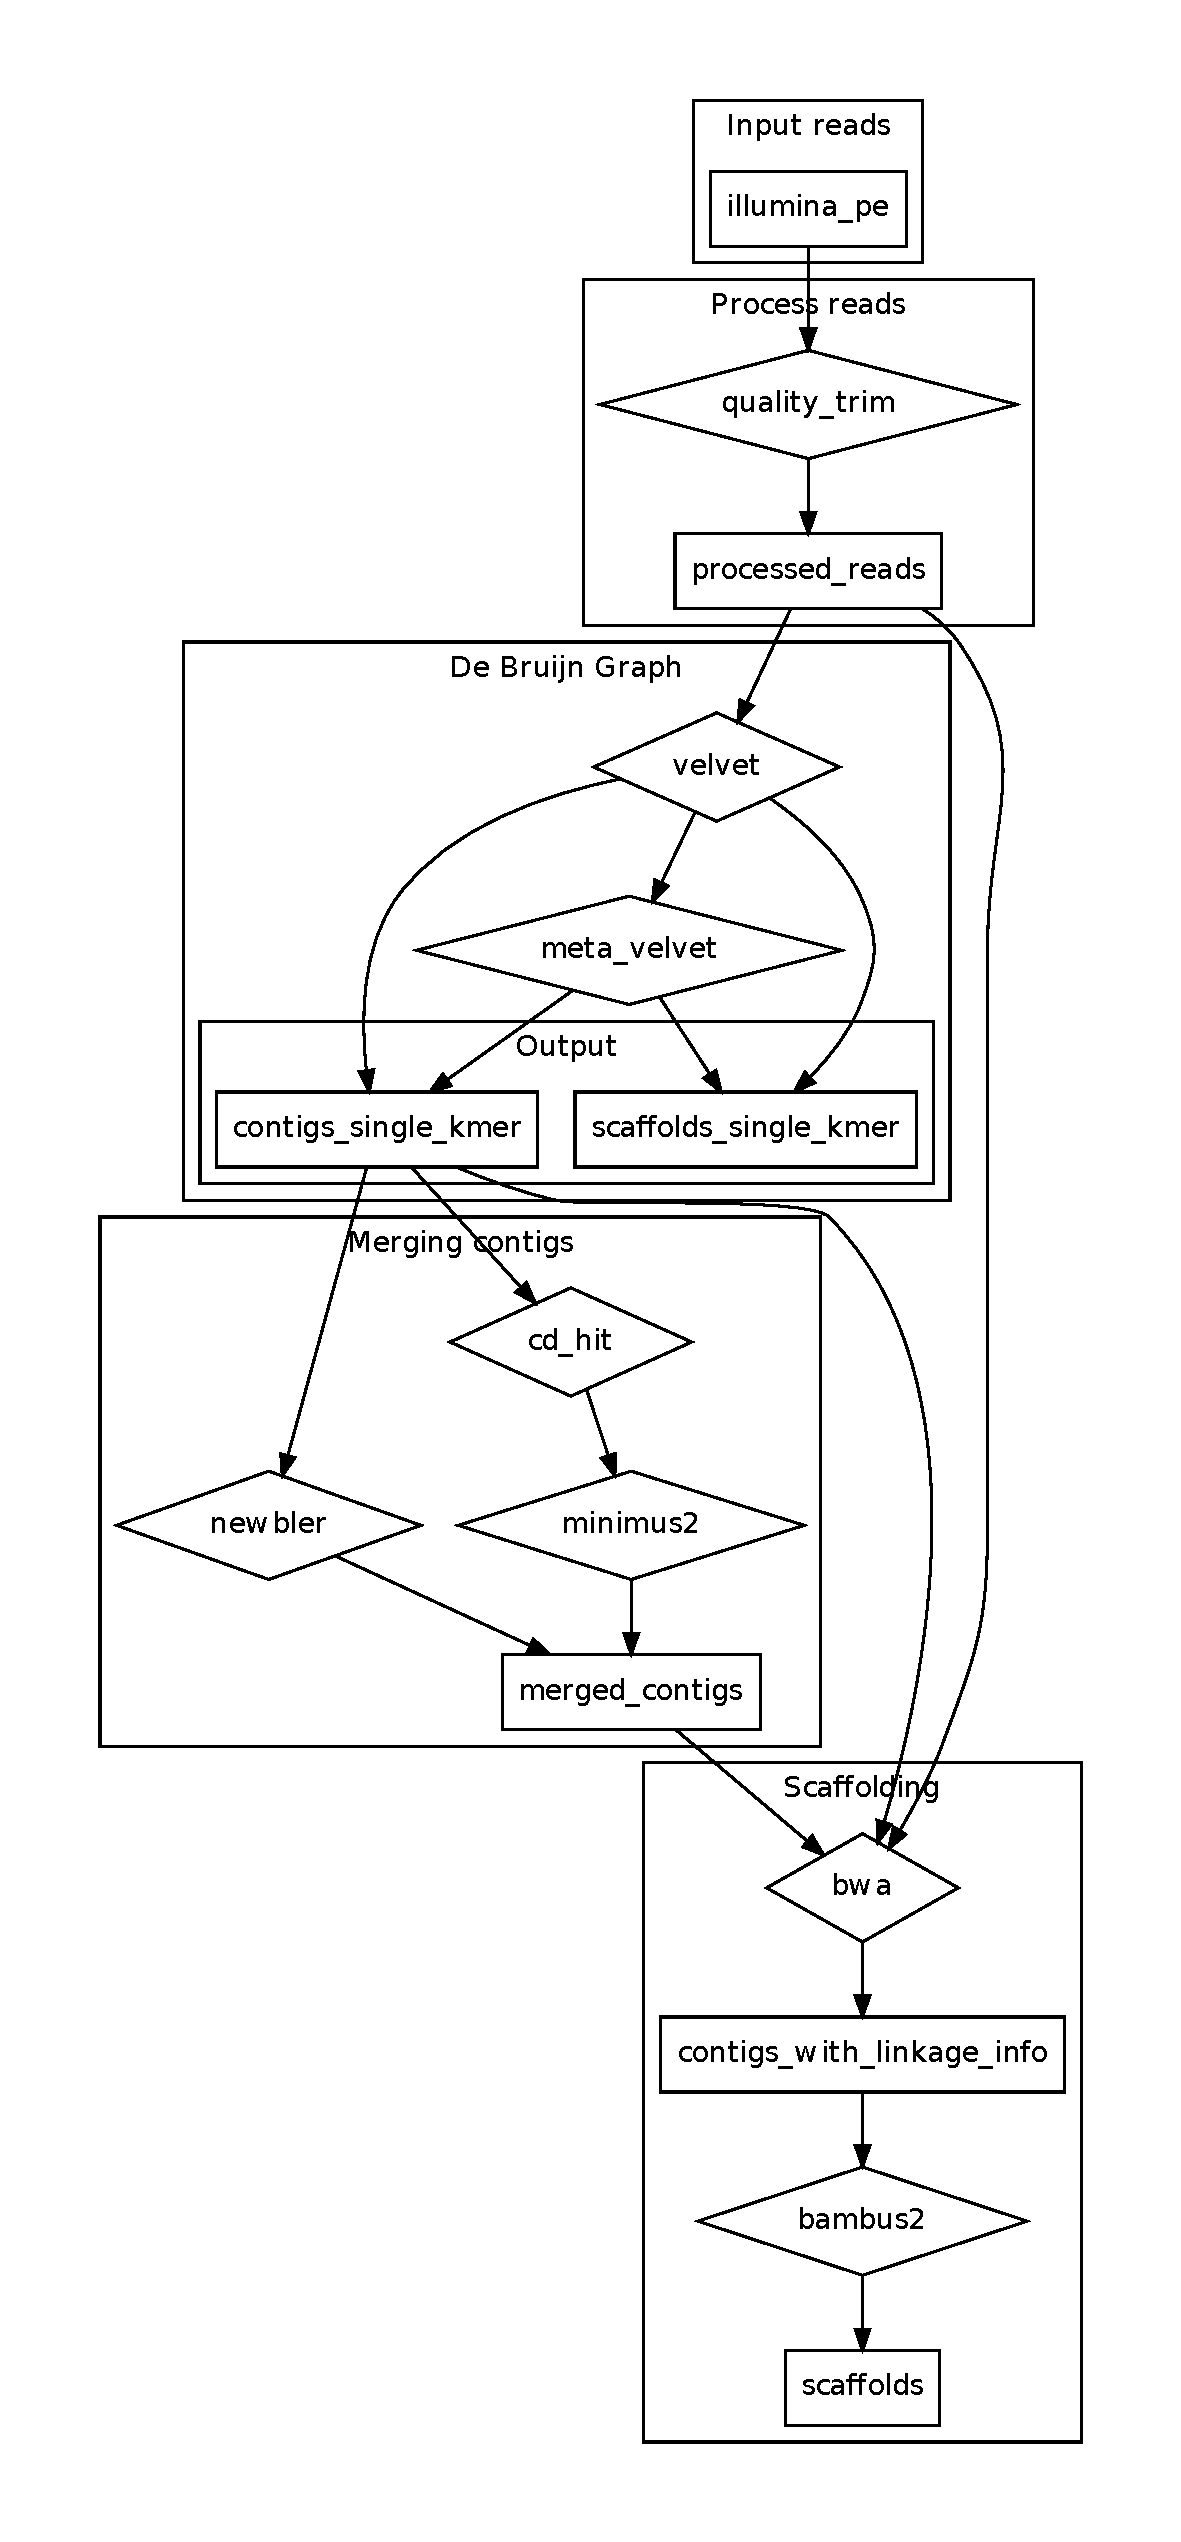
\includegraphics[height=\textheight]{figures/metassemble-flowchart.pdf}
  \caption{Assembly strategies using a combination of Velvet, Meta-Velvet, Ray, Minimus2, Newbler and Bambus2.}
  \label{fig:asmstrat}
\end{figure}

%TODO Validation requires some more non-ambiguous parameters for calculating
% the statistics and performing the mapping with MUMmer

\clearpage \section{Validation} \label{sec:metval} The validation of a metagenomic assembly in
case a reference metagenome is available often focuses on one or more of the
following points:
\begin{itemize}
\item contig or scaffold length distribution
\item contig/scaffold coverage of the reference metagenome
\item chimericity of the contigs/scaffolds
\item functional annotation accuracy
\item phylogenetic classification accuracy
\end{itemize}
This study focusses on the first three points, since those are expected to
improve the functional annotation and the phylogenetic classification.
\citet{Mende22384016} showed that this was indeed the case for functional
annotation.\\


\subsection{Length distribution}
A variety of metrics are used in this validation. For the contig/scaffold
length distribution of an assembly a common metric called the L50 value is
used. L50 is a median value weighted by contig length. Half of all the bases in
the assembly is in contigs equal to or larger than L50.


\subsection{Coverage of the reference metagenome}
\label{sec:cov}
For determining how well the assemblies matched the reference metagenome the
assemblies were mapped against the reference metagenome using MUMmer 3.1
\cite{Kurtz14759262}.  MUMmer finds maximal exact matches longer than $l$ and
clusters them if they are no more than $g$ nucleotides apart. The alignments
are afterwards extended for each cluster if the combined length of its matches
is at least $c$. The alignments are extended in between the matches of the
cluster and on the ends using a Smith-Waterman dynamic programming algorithm.
The MUMmer package contains multiple scripts that make use of this approach.
NUCmer (\underline{NUC}leotide MUM\underline{mer}) is a script included in the
MUMmer package for DNA sequence alignment of a set of query contigs against a
set of reference contigs. The command for NUCmer used was:
\verb!nucmer --maxmatch -c65 -g90 -l20!. The maxmatch parameter makes sure all
exact matches are used, whether they are unique or not, so contigs that consist
only of a shared region or a repetitive element will be included in the
alignments as well. Afterwards the script \verb!show-coords! was used on the
resulting alignment file to extract information about each alignment such as
its location in both the query and the reference, percent identity, percent
similarity and percent of the reference and query covered.\\


To indicate how well the metagenome is covered by the assembled contigs we use
a metric called genome contig coverage and metagenome contig coverage. For each
genome in the reference metagenome, genome contig coverage is determined by
dividing the number of bases that are covered by contigs mapping to it by the
total number of bases in the genome. Metagenome contig coverage is the number
of bases covered by all contigs mapping to it divided by the total number of
bases in the metagenome. In both cases only the best alignment for each contig
is used. The best alignment is the one with the highest purity score (for an
explanation of the purity score see Section \ref{sec:chimer}. In case a contig
aligns equally well to multiple locations, only the first alignment is
considered. This could for instance be a contig that represents a repeat or a
shared region between genomes. By only counting one such alignment not
resolving a repeat or shared region is penalized. Note that in general there's
little difference between counting all such alignments or only one in bacterial
and archaeal genomes \cite{repeat shared region size}.


\subsection{Chimericity}
\label{sec:chimer}
In previous research by \citet{Mavromatis17468765} chimericity of
each contig was determined by the reads mapping to it. This could be done
because reads were selected from finished genome projects, thus 
the origin of each read is known. At each taxonomic level from strain to domain the
contigs were assigned to the phylogenetic group where the majority of reads
stem from. The chimericity was then defined as the number of
reads that belong to another phylogenetic group divided by the total number of
reads mapping to the contig.  \citet{Mende22384016} noted that certain
reads might actually belong to multiple species since there are shared regions between species.
Therefore they proposed a metric called contig score, which is determined by mapping
each contig with blastn to the original genomes, taking the Highest Scoring
Segment Pair (HSP) and multiplying the percent identity times the percent
contig coverage. We use a similar metric, determined with MUMmer
and referred to as purity instead to indicate its relation to chimericity. For
each alignment the purity $p$ is determined by multiplying percent contig
coverage by percent identity divided by 10,000 to get the purity as a ratio
between 0 and 1. The purity of a contig is the maximum purity of all its
alignments. Purity of an entire assembly is computed as well. If $n$ is the
number of contigs, $l_1,...,l_n$ the length of each contig in nucleotides and
$p_1,...,p_n$ the purity of each contig then the global purity $P$ of an entire
assembly is calculated as:

\begin{equation}
P = \frac{\sum_{i=1}^n l_{i} * p_{i}}{\sum_{i=1}^{n} l_{i}}
\end{equation}

For both scaffolds and contigs, only nucleotides are counted when determining
$l$. Thus unknown parts often represented as \verb!N! or \verb!-! do not
contribute to $l$.\\


\section{Pipelines} The vast amount of assemblies and validations that had to
be performed on a variety of libraries gave rise to a need for automation. This
resulted in the development of two pipelines: MetAssemble and MASMVALI
(Metagenomic ASseMbly VALIdation). The former for performing the assemblies,
the latter for validating them given there is a reference metagenome available.

\subsection{MetAssemble}
MetAssemble implements the strategies in Table \ref{tab:asmstrat} and Figure
\ref{fig:asmstrat}. The MetAssemble pipeline was written as a set of rules in
GNU make \cite{GNU make}. GNU make was chosen for a number of reasons:
\begin{itemize}
\item It integrates skipping computation of previously computed files.
    Recomputation is unfortunately only based on modification date, not on the
    actual file contents, but it is good enough for our purposes.
\item GNU make is widely available on Unix and Unix-like systems.
\item After the validation one would want to share only the commands to do a
    specific assembly i.e. not the entire pipeline. Doing a dry-run in GNU make
    gives you the exact commands that generated a certain file.
\end{itemize}
One of the biggest problems in metagenomic assembly are the
computational demands \cite{A practical comparison dada}. The size of the reads
and the number of reads as well as the complexity and the structure of the
sequenced community affect the computational demands. Therefore it is diffcult
to determine the resource usage in advance. In our benchmark several strategies
consist of parts with different computational requirements. Ray for instance
runs over multiple nodes whereas merging with Newbler or Minimus2
requires one node with a lot of memory. Claiming all these computational
resources for the entire run of the pipeline would be a waste. To circumvent
this issue an approach where each step in the pipeline is scheduled as a
separate job using a job scheduler has been chosen. A library was developed for
GNU make to schedule rules as jobs using either sbatch or qsub. The jobs are
scheduled with dependencies on other jobs and the resource usage set for the
rule \cite{link to github}. 

\subsection{MASMVALI}
After the assembly has been completed, the assembly can be validated by
alignment against the reference metagenome. MASMVALI (Metagenomic ASseMbly
VALIdation) is a pipeline written in Python\cite{Python} that calculates the
statistics described in Section \ref{sec:metval}. As minimum input it takes an
assembly, a reference metagenome and alignments found by MUMmer of the
assembly against the reference metagenome. MASMVALI as a pipeline can generate
a HTML report that shows a collection of the plots that are used in this thesis
\cite{github link}. It is also possible to use MASMVALI as a package to do more
analyses on generated assemblies using the available statistics. See for an
example the available ipython notebook \cite{notebook example} \cite{ipython}
\cite{notebook}.

\chapter{Results}

\section{Mock community libraries}
All assemblies in Table \ref{tab:asmstrat} have been performed on the
following libraries:
\begin{description}

\item[50ng even]

    
\includegraphics[width=0.1\textwidth]{figures/logos/even.png}

    Community prepared with 50 ng Nextera library prepartion kit and equal
genome copy numbers. The library has been sequenced with Illumina and contains
$\sim$10M paired reads, each single read has a length of 100.
%\item[500pg even] Community prepared with 500 pg Nextera library prepartion kit and equal
%genome copy numbers.

\item[50ng uneven]

    
\includegraphics[width=0.1\textwidth]{figures/logos/uneven.png}
    
    Community prepared with 50 ng Nextera library prepartion kit
and phyla mixed similar to log-normal distributions of phyla in soil. The
library has been sequenced with Illumina and contains $\sim$10M paired reads,
each single read has a length of 100.
%\item[500pg uneven] Community prepared with 500 pg Nextera library prepartion kit and phyla
%mixed similar to log-normal distributions of phyla in soil.
\end{description}

The original reads of each library were mapped against the reference genome
using BWA \cite{Li20080505} and default values. Afterwards duplicates were
removed with MarkDuplicates from Picard 1.77 (see also Table
\ref{tab:programversions}). In Figure \ref{fig:coverage50ngeven} for the even
library, the even spread of the coverage over all the genomes in the metagenome
can be observed. The median coverage over all bases is 10. The uneven library
covers a couple of genomes very well \ref{fig:coverage50nguneven}. The median
coverage over all bases is 3.\\

\begin{figure}[ht!]
  \centering
    
\includegraphics[width=0.1\textwidth]{figures/logos/even.png}\\
  \centering
      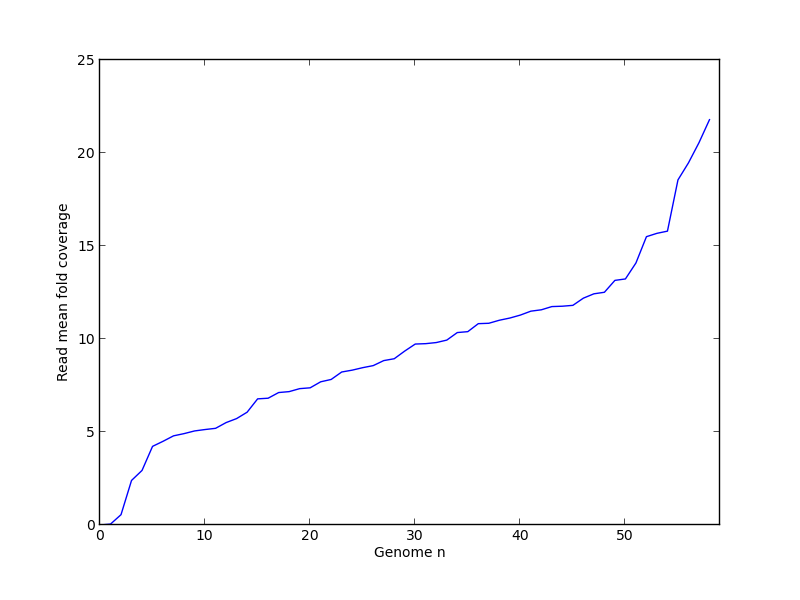
\includegraphics[width=0.8\textwidth,trim=35 20 35 33, clip]{figures/notebooks/chris-mock-even-distribution.png}
  \caption{Read mean coverage of 50ng even per genome. Median coverage over all
  bases is 10.}
  \label{fig:coverage50ngeven}
\end{figure}
\begin{figure}[ht!]
  \centering
    
\includegraphics[width=0.1\textwidth]{figures/logos/uneven.png}\\
  \centering
    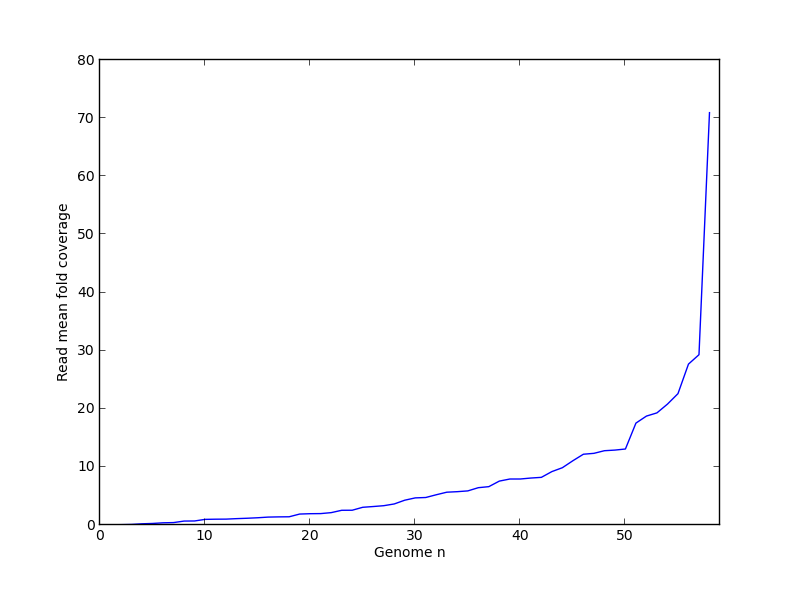
\includegraphics[width=0.8\textwidth,trim=35 20 35 33, clip]{figures/notebooks/chris-mock-uneven-distribution.png}
  \caption{Read mean coverage of 50ng uneven per genome. Median coverage over
  all bases is 3.}
  \label{fig:coverage50nguneven}
\end{figure}


\section{Length distribution}
\label{res:len}
\begin{figure}[ht!]
  \centering
    
\includegraphics[width=0.1\textwidth]{figures/logos/even.png}
    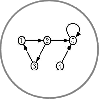
\includegraphics[width=0.1\textwidth]{figures/logos/contig.png}\\
  \centering
    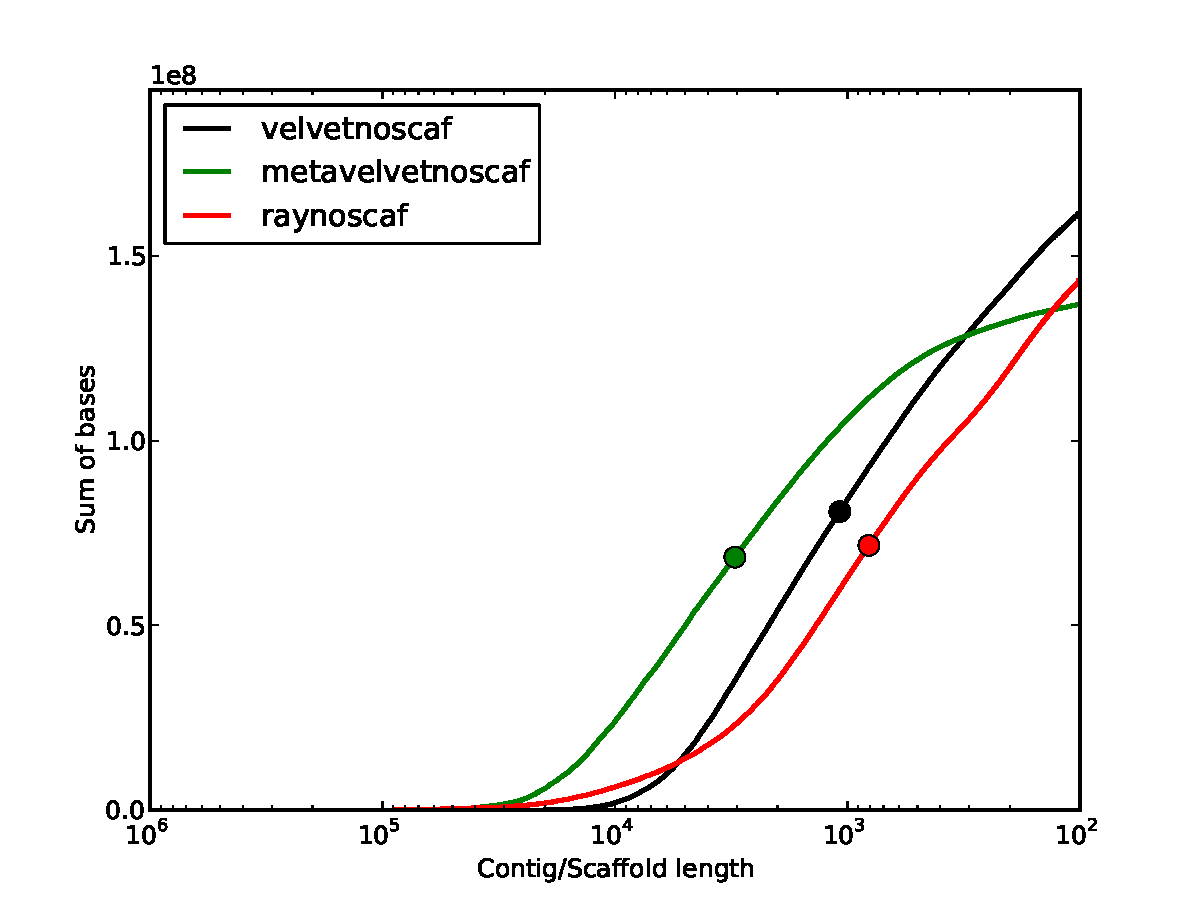
\includegraphics[width=0.8\textwidth,trim=35 20 35 33, clip]{figures/notebooks/chris-mock-length-distribution/even-contig.pdf}
  \caption{Length distribution comparison of different contiging strategies.
      Sum of bases shown as a function of contig length, x-axis is log-scaled
      and inverted. }
  \label{fig:length-distribution-even-contig-length}
\end{figure}

In Figure \ref{fig:length-distribution-even-contig-length} the length
distribution of the contiging strategies are shown. Each plotted line
represents one assembly. The dots indicate L50 values on the x-axis. The assemblies are based on
reads from the even library. For each assembly strategy the assembly with a
kmer that resulted in the highest L50 has been chosen. For {\em velvetnoscaf}
and {\em metavelvetnoscaf} $k=25$, for Ray $k=21$. Meta-Velvet scores the
highest on L50, but not only by combining contigs not combined by Velvet.  It
actually also removes a lot of short contigs from the original Velvet assembly,
resulting in a lower total sum of bases. Depending on what size of contigs are
required for the post post-processing the winner differs. Longer than 100,
Velvet and to a lesser extent Ray give more total bases, but longer than 1000
Meta-Velvet would seem a better candidate. When comparing length distributions
between different assemblers, only looking at L50 is thus not enough. Only to
compare length distributions between assemblies stemming from the same assembly
strategy L50 can be used.\\

In Figure \ref{fig:chris-mock-length-distribution-roc} all assembly strategies
are compared over length distributions. On the x-axis are contig numbers where
contigs in each assembly are numbered by size from largest to smallest. In the
first row that shows the contiging strategies, the uneven sample increases the
gap in sum of bases between Meta-Velvet and the other assemblers even more. The
merging strategies increase lengths quite significantly for both libraries. The
difference between Newbler and Minimus2 being rather small. Minimus2 results in
slightly larger contigs, whereas Newbler reaches a higher sum in some cases.
The internal scaffolding options of the assemblers improves lengths, but the
sum of bases decreases substantially.  For the external scaffolder, Bambus2,
the sum decreases even more.\\


Notice also how the internal scaffolder from Meta-Velvet and Velvet result in
the same assembly for the even library. Meta-Velvet is based on following
multiple peaks in the coverage distribution where each peak would theoretically
represent an organism. Velvet can follow one peak with the \verb!-exp_cov auto!
parameter. For the contiging approach however this parameter is not set (See
Table \ref{tab:asmstratparameters}), but for Meta-Velvet it is, which results
in different assemblies for the even library.  To enable internal scaffolding
in Velvet one has to set the \verb!-exp_cov auto!  parameter, making Velvet and
Meta-Velvet follow the same peak in coverage for the even library. For the
uneven library the results differ, since Meta-Velvet finds multiple peaks and
Velvet only uses one. 


\section{Metagenome coverage}
In Figure \ref{fig:chris-mock-length-distribution-cov-roc} the sum of bases
axes from Figure \ref{fig:chris-mock-length-distribution-roc} have been
replaced by the metagenome coverage. The actual non-overlapping contig coverage
of the reference metagenome after adding a particular contig (see Section
\ref{sec:cov}).  An addition of a contig that doesn't increase the metagenome
coverage by its own length could be due to:
\begin{enumerate}
\item\label{en:aln} the contig not aligning anywhere
\item\label{en:chi} the contig aligns only partially because it is chimeric or has errors
\item\label{en:dup} the mapping location is already partially or fully covered by another
contig.
\end{enumerate}
Overal the plots look very similar to the original length distributions.  The
increase in coverage is less smooth than the increase in length indicating that
one or more of the three previously mentioned points occur, but not in an
extreme fashion. In case no reference metagenome is available looking at the
length distributions in this manner is thus a good indication of the metagenome
coverage.\\


We found that nearly all contigs for each assembly are aligning \cite{table??}.
None of the assemblers thus creates invalid contigs. Whether point \ref{en:chi}
or \ref{en:dup} is the case is shown in Section \ref{sec:reschi} for the
different assembly strategies.


% One page figure over length distributions roc style
\onepagecmp{chris-mock-length-distribution}{A comparison of assembly
strategies on length distributions. Contigs ordered by numbering from longest
to shortest.}

\onepagecmp{chris-mock-length-distribution-cov}{A comparison of assembly
strategies on metagenome coverage. Contigs ordered by numbering from longest to
shortest.}

\section{Chimericity}
\label{sec:reschi}
To determine the chimericty of the contigs in an assembly the global purity
metric described in Section \ref{sec:metval} is used. In Figure \ref{??} 
all assemblies are compared on purity where global purity is shown as a
function of L50. In this plot every dot represents a single assembly. The size
of the dot represents the kmer size from 19 to 75. Although a high L50 is not a
perfect indication of a good length distribution, it does allow one to see how
increases in length are related to the chimericity of the contigs in the
assembly. The L50 values are all based on a cut-off length of 100.\\


The contiging strategies display a minor decrease in purity for an increase in
L50 with shorter $k$. There is always some point visible for the Meta-Velvet
assemblies where the L50 goes down again with a too short $k$. At that point
the de Bruijn graph becomes saturated with too many connections. This point
occurs between $k=20$ and $k=30$ for all three assemblers although for Velvet
and Ray it is not clearly visible from the graph. The even community results in
a more continuous line with varying $k$ than the uneven library for
Meta-Velvet. For the uneven library some clusters are visible. No cause for
these clusters has been researched, but a possible explanation is that it has
to do with the way Meta-Velvet selects the coverage peaks, since that is a
binary choice. At a certain $k$ the coverage threshold is reached and a peak is
detected, which could give rise to the clusters in the plot.\\


The merging strategies perform well, the L50 is increased and the purity is
kept high. The Newbler assemblies are only slightly purer than Minimus2 in some
cases. Therefore the bigger bigger contig lengths of Minimus2 compared to the
metagenome coverage in Figure \ref{chris-mock-length-distribution-cov-roc} are
probably due to duplicate contigs.\\


The internal scaffolding introduces a lot of unpure contigs. Notice also how
Ray's internal scaffolder decreases in purity with decreasing $k$, whereas
Velvet and Meta-Velvet have increased purity with decreasing $k$. At the lower
values of $k$ the purity is very similar. Bambus2 results in very pure
assemblies. As demonstrated in Section \ref{res:len} the larger L50 values
compared to the other assembly stategies is in large part a result of losing
many short contigs.\\


\onepagecmp{chris-mock-purity-l50-asm-stats}{A comparison of assembly
strategies on purity.}

\chapter{Discussion}
It is difficult to name one true winner. Depending on the post-processing and
the computational resources available the most suitable assembly strategy
differs. In case one is only interested in post-processing contigs larger than
1K, Meta-Velvet performs well. Larger than 100: Velvet is a suitable
candidates. For large libraries that would require too much memory to run
Velvet, Ray can be used. In general the merging strategies preform well on all
three validated properties: length, metagenome coverage and purity. There are
minor differences between using either Newbler or Minimus2 for merging.
Minimus2 results in more duplication. So even though both mergers do not make
use of metagenomic heuristics they perform well. A merger that does implement
the use of all the information available, such as the read coverage of the
contigs and pair linkage between contigs seems like a worthwhile project.\\


The current results are only based on two libraries so future work of doing the
same analysis on another library and the same or a different mock community
would give more insight whether the conclusions hold in other circumstances.
Ideally one could get an insight for each type of community what assembly
strategy is preferred. Making the analysis in this paper available as a web
service allowing users to run it on their own assembly, library, mock community
combination and comparing them to the existing ones, could lead to a form of
crowdsourced benchmarking.\\


The post-processing steps such as taxonomic classification and gene annotation
have not been part of this study. It would be significant to know what size of
contigs can be used in these post-processing steps and what purity level is
required. Is there a balance between length increase and purity loss that is
benificial for a certain type of post-processing?\\


Our efforts have focussed on validating assemblies when a reference is
available. Apart from the length distribution plot that is a decent indication
of metagenome coverage, no reference-less validation approaches have been
suggested. Comparing our results versus a reference-less validation technique,
such as Feature Response Curve \cite{TODO} or ALE \cite{TODO} would be a an
important addition, especially since metagenomics rose out of the problem that
the vast majority of microbes cannot be cultured in the lab.


%Low coverage libraries
%Future work from presentation


%\clearpage
%\begin{landscape}
%\begin{figure}[ht]
%\noindent
%\centering
%\begin{minipage}{\textheight}
%    \hspace*{0.21\textheight}
%    \centering
%    \raisebox{-0.5\height}{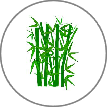
\includegraphics[width=0.1\textheight]{figures/logos/bambus2.png}}
%    \hspace*{0.01\textheight}
%    \centering
%    \raisebox{-0.5\height}{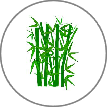
\includegraphics[width=0.1\textheight]{figures/logos/bambus2.png}}
%    \hspace*{0.01\textheight}
%    \centering
%    \raisebox{-0.5\height}{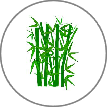
\includegraphics[width=0.1\textheight]{figures/logos/bambus2.png}}
%    \hspace*{0.01\textheight}
%    \centering
%    \raisebox{-0.5\height}{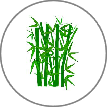
\includegraphics[width=0.1\textheight]{figures/logos/bambus2.png}}
%    \hspace*{0.01\textheight}
%    \centering
%    \raisebox{-0.5\height}{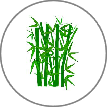
\includegraphics[width=0.1\textheight]{figures/logos/bambus2.png}}
%    \hspace*{0.01\textheight}
%\end{minipage}\\
%\begin{minipage}{\textheight}
%    \centering
%    \raisebox{-0.5\height}{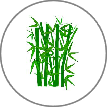
\includegraphics[width=0.2\textheight]{figures/logos/bambus2.png}}
%    \hspace*{0.01\textheight}
%    \centering
%    \raisebox{-0.5\height}{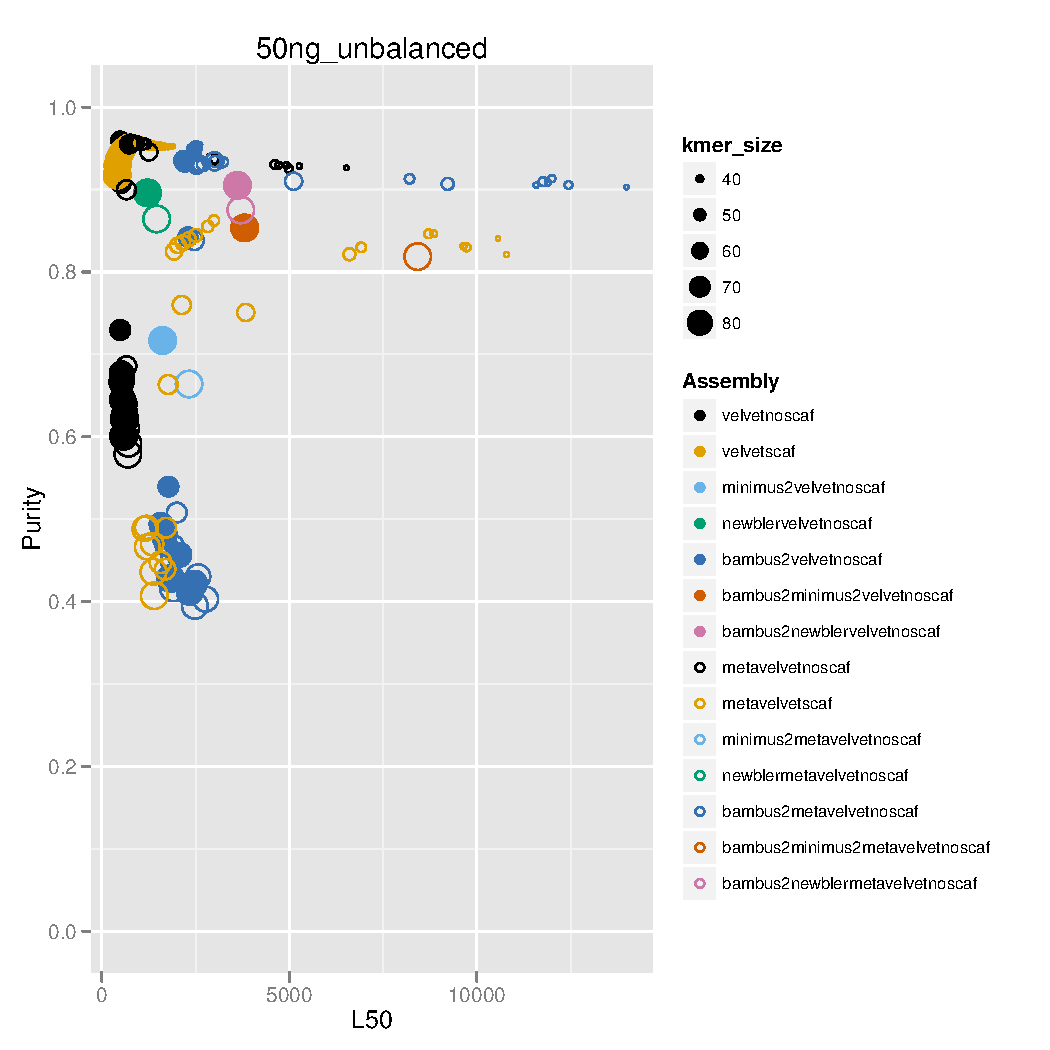
\includegraphics[width=0.2\textheight]{figures/l50-purity-50ng_unbalanced.pdf}}
%    \hspace*{0.01\textheight}
%    \centering
%    \raisebox{-0.5\height}{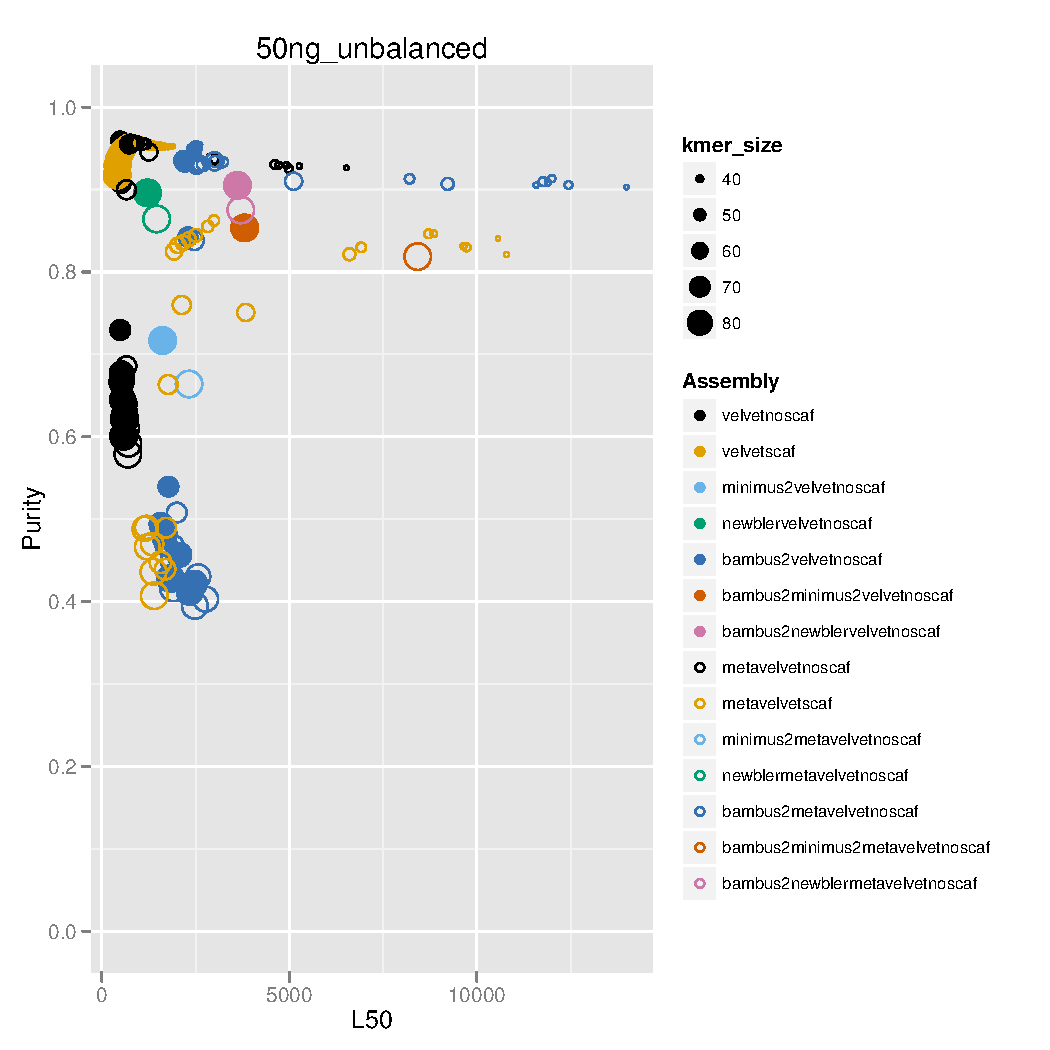
\includegraphics[width=0.2\textheight]{figures/l50-purity-50ng_unbalanced.pdf}}
%    \hspace*{0.01\textheight}
%    \centering
%    \raisebox{-0.5\height}{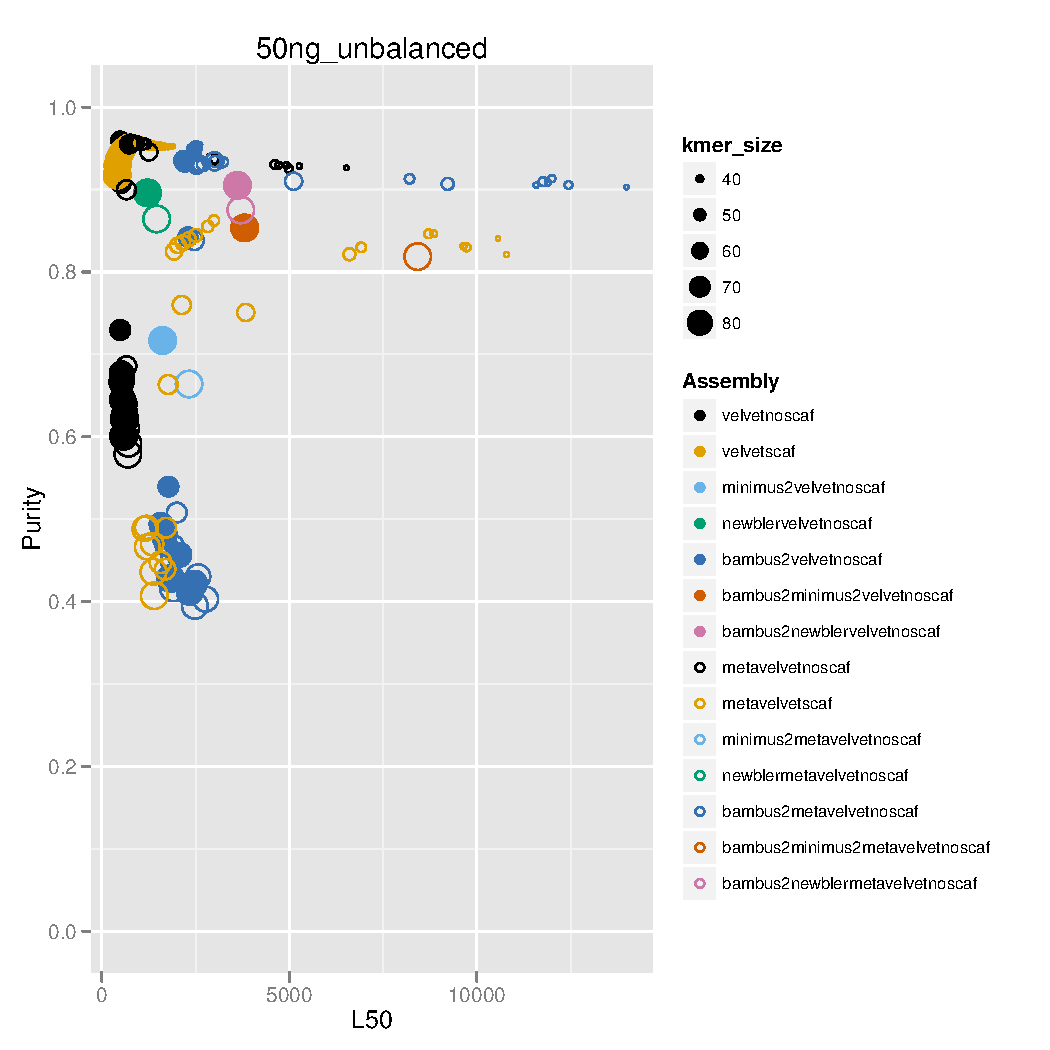
\includegraphics[width=0.2\textheight]{figures/l50-purity-50ng_unbalanced.pdf}}
%    \hspace*{0.01\textheight}
%    \centering
%    \raisebox{-0.5\height}{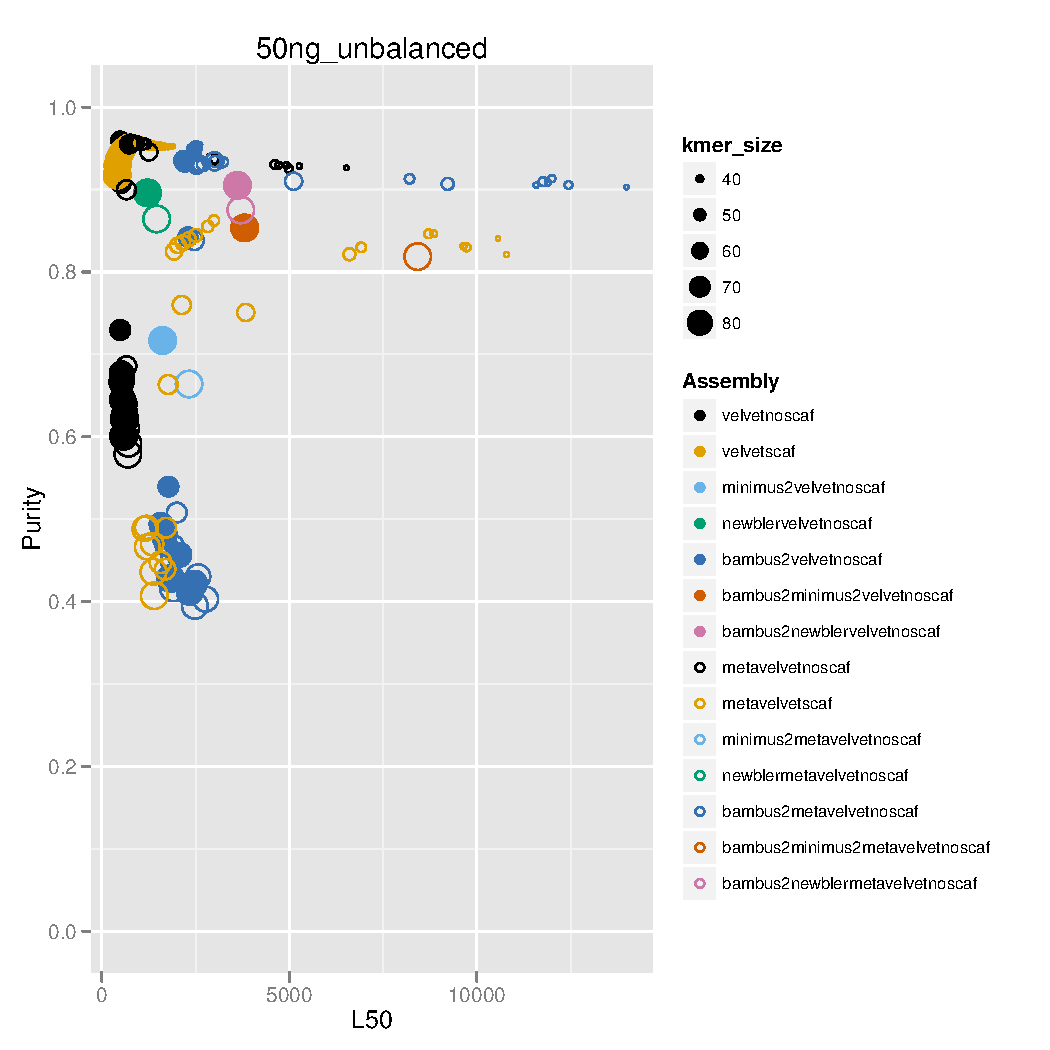
\includegraphics[width=0.2\textheight]{figures/l50-purity-50ng_unbalanced.pdf}}
%    \hspace*{0.01\textheight}
%    \centering
%    \raisebox{-0.5\height}{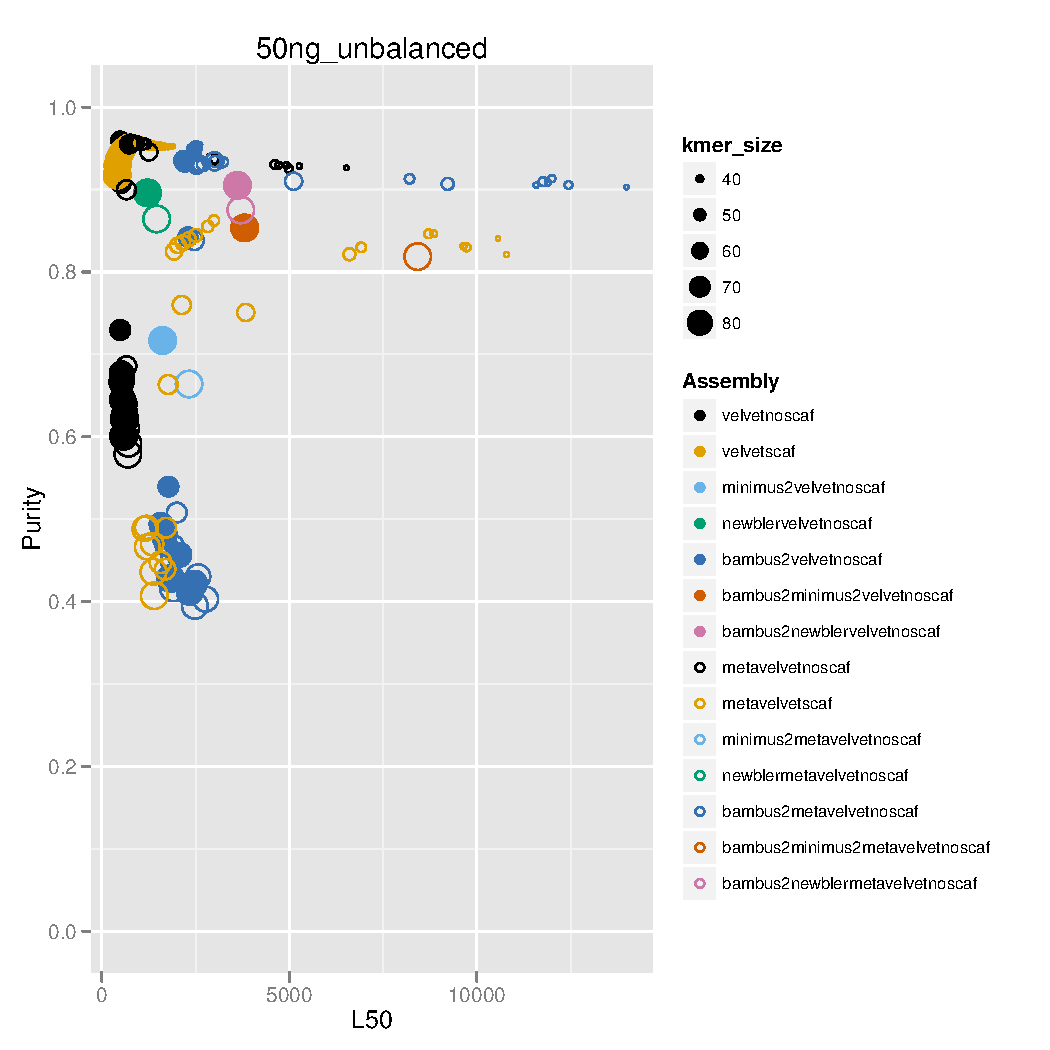
\includegraphics[width=0.2\textheight]{figures/l50-purity-50ng_unbalanced.pdf}}
%\end{minipage}
%\caption{All that jazz}
%\end{figure}
%\end{landscape}
%\clearpage

\clearpage
%\bibliographystyle{report.bst}
\bibliographystyle{plainnat}
\bibliography{report}

% Supplementary section
\appendix
\clearpage
\pagestyle{empty}
\newgeometry{bottom=3cm}
\begin{landscape}
\footnotesize
\begin{table}[htbp]
\begin{tabular}{|l|r|p{9cm}|}
\hline
Program & Version & URL \\ \hline
sickle & commit 2013-4-3 e435598aa6bbb74b3254d2884a9dea1b0639d464 & \url{https://github.com/najoshi/sickle} \\ \hline
Velvet & 1.2.01 & \url{https://github.com/dzerbino/velvet/commit/5d5b636c52e94fde745cb8bf753ffa134126e04d} \\ \hline
Meta-Velvet & 1.2.01 &  \\ \hline
Minimus2 & Amos commit 2012-3-6 & \url{http://amos.git.sourceforge.net/git/gitweb.cgi?p=amos/amos;a=commit;h=7c70d6c36dba244ae0b266fc52a5206ab202a36c} \\ \hline
Newbler & RunAssembly 2.6 (20110517\_1502) &  \\ \hline
MUMmer & 3.23 & \url{http://sourceforge.net/projects/mummer/files/mummer/3.23/MUMmer3.23.tar.gz/download} \\ \hline
CD-HIT & 4.5.7 & \\ \hline
Picard & 1.77 & \\ \hline
bwa & 0.6.1-r104 & \\ \hline
Bambus2 & Amos commit 2012-3-6 & \url{http://amos.git.sourceforge.net/git/gitweb.cgi?p=amos/amos;a=commit;h=7c70d6c36dba244ae0b266fc52a5206ab202a36c} \\ \hline
samtoafg & Amos commit 2012-3-6 & \url{http://amos.git.sourceforge.net/git/gitweb.cgi?p=amos/amos;a=commit;h=7c70d6c36dba244ae0b266fc52a5206ab202a36c} \\ \hline 
Ray & 2.1.0 & \url{http://denovoassembler.sourceforge.net/} \\ \hline
\end{tabular}
\caption{Program versions used for the analysis}
\label{tab:programversions}
\end{table}
\end{landscape}


\clearpage
\begin{landscape}
\begin{table}[h!]
\begin{tabular}{|l|p{17cm}|}
\hline
Assembly strategy name & Program Parameters\\
\hline
velvetnoscaf & Run \verb!velveth $dir 31,84,2 -fastq -shortPaired $pairs.fastq! and run \verb!velvetg -scaffolding no! on the resulting directories.\\\hline
velvetscaf & Run \verb!velveth $dir 31,84,2 -fastq -shortPaired $pairs.fastq! and run \verb!velvetg -scaffolding yes -exp_cov auto! on the resulting directories.\\\hline
metavelvetnoscaf & Run \verb!velveth $dir 31,84,2 -fastq -shortPaired $pairs.fastq! and run \verb!velvetg -scaffolding no -exp_cov auto -read_trkg yes && -scaffolding no! on the resulting directories.\\\hline
metavelvetscaf & Run \verb!velveth $dir 31,84,2 -fastq -shortPaired $pairs.fastq! and run \verb!velvetg -scaffolding no -exp_cov auto -read_trkg yes && -scaffolding yes! on the resulting directories.\\\hline
raynoscaf & Run \verb!Ray -k $kmersize -i $pairs.fastq -o output_dir!.\\\hline
minimus2* & Concatenate contigs larger than 200 and run \newline\verb!cd-hit-est -c 0.99 -i $concat.fasta -o $derep.fasta! to remove similar sequences. Run \verb!toAmos -s $derep.fasta -o $derep.afg! followed by \verb!minimus2 $derep!. From \url{http://ged.msu.edu/angus/metag-assembly-2011/velvet-multik.html} \\\hline
newbler* & Cut all contigs up in chunks of 1999 bases with an overlap of 1900 bases and run\newline \verb!runAssembly -o $dir $cut-up-contigs.fasta!. From \cite{Luo22347999}. \\\hline
bambus2* & Map paired reads with \verb!bwa! using default parameters to contigs and remove duplicate reads with \verb!MarkDuplicates!. Run \verb!samtoafg! to convert to afg, import to Amos bnk with \verb!bank-transact! and finally run \verb!goBambus2!.\\\hline
\hline
\end{tabular}
\caption{Program parameters per assembly strategy.}
\label{tab:asmstratparameters}
\end{table}
\end{landscape}

\clearpage
\begin{landscape}
\begin{center}
\footnotesize
\begin{longtable}{|r|l|c|l|l|l|}
\caption{Mock community}\label{tab:mock}\\
\hline
No & Genome Name & Genome Size (bp) & Domain & Phylum & Class \\

\hline
\endfirsthead
\multicolumn{6}{c}%
{{\bfseries \tablename\ \thetable{} Mock Community -- continued from previous page}} \\
\hline
No & Genome Name & Genome Size (bp) & Domain & Phylum & Class \\
\hline
\endhead

\hline \multicolumn{6}{|r|}{{Continued on next page}} \\ \hline
\endfoot

\hline 
\endlastfoot
1 & Acidobacterium capsulatum ATCC 51196 & 4127356 & Bacteria & Acidobacteria & Acidobacteriae \\
2 & Akkermansia muciniphila ATCC BAA-835 & 2664102 & Bacteria & Verrucomicrobia & Verrucomicrobiae \\
3 & Anaerocellum thermophilum Z-1320, DSM 6725 & 2919718 & Bacteria & Firmicutes & Clostridia \\
4 & Bacteroides thetaiotaomicron VPI-5482 & 6293399 & Bacteria & Bacteroidetes & Bacteroidia \\
5 & Bacteroides vulgatus ATCC 8482 & 5163189 & Bacteria & Bacteroidetes & Bacteroidia \\
6 & Bordetella bronchiseptica RB50 & 5339179 & Bacteria & Proteobacteria & Betaproteobacteria \\
7 & Burkholderia xenovorans LB400 & 973113 & Bacteria & Proteobacteria & Betaproteobacteria \\
8 & Caldicellulosiruptor saccharolyticus DSM 8903 & 2970275 & Bacteria & Firmicutes & Clostridia \\
9 & Chlorobaculum tepidum TLS & 2154946 & Bacteria & Chlorobi & Chlorobia \\
10 & Chlorobium limicola DSM 245 & 2763181 & Bacteria & Chlorobi & Chlorobia \\
11 & Chlorobium phaeobacteroides DSM 266 & 3133902 & Bacteria & Chlorobi & Chlorobia \\
12 & Chlorobium phaeovibrioides DSM 265 & 1966858 & Bacteria & Chlorobi & Chlorobia \\
13 & Chloroflexus aurantiacus J-10-fl & 5258541 & Bacteria & Chloroflexi & Chloroflexi \\
14 & Clostridium thermocellum ATCC 27405 & 3843301 & Bacteria & Firmicutes & Clostridia \\
15 & Deinococcus radiodurans R1 & 3284156 & Bacteria & Thermi & Deinococci \\
16 & Desulfovibrio desulfuricans desulfuricans ATCC 27774 & 2873437 & Bacteria & Proteobacteria & Deltaproteobacteria \\
17 & Desulfovibrio piger ATCC 29098 & 2826240 & Bacteria & Proteobacteria & Deltaproteobacteria \\
18 & Dictyoglomus turgidum DSM 6724 & 1855560 & Bacteria & Dictyoglomi & Dictyoglomia \\
19 & Enterococcus faecalis V583 & 3359974 & Bacteria & Firmicutes & Bacilli \\
20 & Fusobacterium nucleatum nucleatum ATCC 25586 & 2174500 & Bacteria & Fusobacteria & Fusobacteria \\
21 & Gemmatimonas aurantiaca T-27T & 4636964 & Bacteria & Gemmatimonadetes & Gemmatimonadetes \\
22 & Herpetosiphon aurantiacus ATCC 23779 & 6785430 & Bacteria & Chloroflexi & Chloroflexi \\
23 & Hydrogenobaculum sp. Y04AAS1 & 1559514 & Bacteria & Aquificae & Aquificae \\
24 & Leptothrix cholodnii SP-6 & 4909403 & Bacteria & Proteobacteria & Betaproteobacteria \\
25 & Nitrosomonas europaea ATCC 19718 & 2812094 & Bacteria & Proteobacteria & Betaproteobacteria \\
26 & Nostoc sp. PCC 7120 & 7211789 & Bacteria & Cyanobacteria & unclassified \\
27 & Pelodictyon phaeoclathratiforme BU-1 & 3018238 & Bacteria & Chlorobi & Chlorobia \\
28 & Persephonella marina EX-H1 & 2467104 & Bacteria & Aquificae & Aquificae \\
29 & Porphyromonas gingivalis ATCC 33277 & 2354886 & Bacteria & Bacteroidetes & Bacteroidia \\
30 & Rhodopirellula baltica SH 1 & 7145576 & Bacteria & Planctomycetes & Planctomycetacia \\
31 & Rhodospirillum rubrum ATCC 11170 & 4406557 & Bacteria & Proteobacteria & Alphaproteobacteria \\
32 & Ruegeria pomeroyi DSS-3 & 4601053 & Bacteria & Proteobacteria & Alphaproteobacteria \\
33 & Salinispora arenicola CNS-205 & 5786361 & Bacteria & Actinobacteria & Actinobacteria \\
34 & Salinispora tropica CNB-440 & 5183331 & Bacteria & Actinobacteria & Actinobacteria \\
35 & Shewanella baltica OS185 & 5312910 & Bacteria & Proteobacteria & Gammaproteobacteria \\
36 & Shewanella baltica OS223 & 5358884 & Bacteria & Proteobacteria & Gammaproteobacteria \\
37 & Sulfitobacter sp. EE-36 & 3547243 & Bacteria & Proteobacteria & Alphaproteobacteria \\
38 & Sulfitobacter sp. NAS-14.1 & 4002069 & Bacteria & Proteobacteria & Alphaproteobacteria \\
39 & Sulfurihydrogenibium sp. YO3AOP1 & 1838442 & Bacteria & Aquificae & Aquificae \\
40 & Sulfurihydrogenibium yellowstonense SS-5 & 1534471 & Bacteria & Aquificae & Aquificae \\
41 & Thermoanaerobacter pseudethanolicus ATCC 33223 & 2362816 & Bacteria & Firmicutes & Clostridia \\
42 & Thermotoga neapolitana DSM 4359 & 1884562 & Bacteria & Thermotogae & Thermotogae \\
43 & Thermotoga petrophila RKU-1 & 1824357 & Bacteria & Thermotogae & Thermotogae \\
44 & Thermotoga sp. RQ2 & 1877693 & Bacteria & Thermotogae & Thermotogae \\
45 & Thermus thermophilus HB8 & 2116056 & Bacteria & Thermi & Thermi \\
46 & Treponema denticola ATCC 35405 & 2843201 & Bacteria & Spirochaetes & Spirochaetes \\
47 & Wolinella succinogenes DSM 1740 & 2110355 & Bacteria & Proteobacteria & Epsilonproteobacteria \\
48 & Zymomonas mobilis mobilis ZM4 & 2223497 & Bacteria & Proteobacteria & Alphaproteobacteria \\
49 & Archaeoglobus fulgidus DSM 4304 & 2178400 & Archaea & Euryarchaeota & Archaeoglobi \\
50 & Ignicoccus hospitalis KIN4/I & 1297538 & Archaea & Crenarchaeota & Thermoprotei \\
51 & Methanocaldococcus jannaschii DSM 2661 & 1 664 970 & Archaea & Euryarchaeota & Methanococci \\
52 & Methanococcus maripaludis C5 & 1 780 761 & Archaea & Euryarchaeota & Methanococci \\
53 & Methanococcus maripaludis S2 & 1 661 137 & Archaea & Euryarchaeota & Methanococci \\
54 & Nanoarchaeum equitans Kin4-M & 490 885 & Archaea & Nanoarchaeota & Nanoarchaea \\
55 & Pyrobaculum aerophilum IM2 & 2 222 430 & Archaea & Crenarchaeota & Thermoprotei \\
56 & Pyrobaculum calidifontis JCM 11548 & 2 009 313 & Archaea & Crenarchaeota & Thermoprotei \\
57 & Pyrococcus horikoshii OT3 & 1 738 505 & Archaea & Euryarchaeota & Thermococci \\
58 & Sulfolobus tokodaii 7(S311) & 2 694 756 & Archaea & Crenarchaeota & Thermoprotei \\
59 & Treponema vincentii I & 2512734 & Bacteria & Spirochaetes & Spirochaetia \\
%60 & Erwinia chrysanthemi & 3909000 & Bacteria & Proteobacteria; & Gammaproteobacteria \\
\end{longtable}
\end{center}
\end{landscape}


\end{document}
